\clearpage
\section{Follow-up Target Controls}
\label{app:followup_controls}
The follow-up covers CIFAR-100N base seed 44 and CIFAR-10N Worse base seed 43. It reuses frozen base features, the original train-only PCA, and the nine existing base-feature heads per base. Three new heads per base predict the mean observed-label margin over five augmentations at the minimum-noisy-validation-loss checkpoint. The transform is the actual base-training sequence: constant-padding random crop at $32\times32$, random horizontal flip, then ImageNet resize/normalization. This differs from the reflected-padding inference-view stream. Original training RNG draws were not recorded; the control samples new deterministic draws (seed 20261019). It neither matches online weight evolution nor separates the cross-entropy warmup from later GCE training.

All old validation-selected policies and downstream accuracy values reproduce. New policies freeze before test evaluation; clean training labels do not construct targets or fit heads. The two augmentation-control jobs together fit six new heads; no base is retrained. The complete follow-up batch, including direct comparisons and runtime measurements, takes 41.89 minutes. This is not the cost of one deployment head.

\begin{table}[!ht]
\centering\small
\caption{Follow-up accuracy (\%); mean $\pm$ sample SD over three heads on each base. Each method retains its own noisy-validation-selected policy.}
\label{tab:followup_accuracy}
\begin{tabular}{lrrr}
\toprule
Target & Base 42 & Base 43 & Base 44 \\
\midrule
\multicolumn{4}{l}{\textbf{CIFAR-100N}} \\
Static & 70.35 $\pm$ 0.10 & 69.27 $\pm$ 0.01 & 69.57 $\pm$ 0.00 \\
Aug-static & 70.32 $\pm$ 0.04 & 69.27 $\pm$ 0.02 & 69.57 $\pm$ 0.00 \\
History-50 & 70.46 $\pm$ 0.18 & 69.93 $\pm$ 0.09 & 69.68 $\pm$ 0.18 \\
Early-5 & 71.08 $\pm$ 0.24 & 70.28 $\pm$ 0.13 & 70.09 $\pm$ 0.21 \\
\multicolumn{4}{l}{\textbf{CIFAR-10N Worse}} \\
Static & 89.19 $\pm$ 0.13 & 90.53 $\pm$ 0.02 & 88.82 $\pm$ 0.10 \\
Aug-static & 89.28 $\pm$ 0.08 & 90.61 $\pm$ 0.05 & 88.91 $\pm$ 0.07 \\
History-50 & 89.01 $\pm$ 0.31 & 90.43 $\pm$ 0.12 & 89.35 $\pm$ 0.19 \\
Early-5 & 90.16 $\pm$ 0.02 & 91.28 $\pm$ 0.02 & 90.39 $\pm$ 0.15 \\
\bottomrule
\end{tabular}

\end{table}

Table~\ref{tab:followup_pairs} gives direct Early-5 minus reference contrasts for the base-feature heads. Accuracy intervals use 2,000 paired test-example draws. AUROC differences compare original-view scores against the same original-view base-error events; their intervals use 2,000 paired stratified draws retaining the observed error/correct counts, with bootstrap seed 20261019. They are nominal, conditional, exploratory intervals without multiplicity correction, not intervals over independently trained bases.

For Early-5 versus augmented-static, CIFAR-100N head-42/43/44 AUROC differences are 0.0259, 0.0260 and 0.0320, with intervals $[0.0198,0.0325]$, $[0.0195,0.0323]$, and $[0.0256,0.0383]$. CIFAR-10N differences are 0.0183, 0.0186 and 0.0168, with intervals $[0.0123,0.0239]$, $[0.0130,0.0238]$, and $[0.0107,0.0229]$. These positive ranking differences do not guarantee accuracy improvements or calibrated probabilities.

\begin{table}[!ht]
\centering\scriptsize
\caption{Direct paired target contrasts. Gain and CI are accuracy percentage points; $\Delta$AUROC refers to original-view error ranking. $V_r/V_e$ lists reference/Early-5 selected views.}
\label{tab:followup_pairs}
\begin{tabular}{lllrrrr}
\toprule
Run & Seed & Reference & $V_r/V_e$ & Gain & 95\% CI & $\Delta$AUROC \\
\midrule
C100/44 & 42 & Static & 1/5 & +0.53 & [+0.00, +1.04] & +0.0214 \\
C100/44 & 42 & History-50 & 5/5 & +0.42 & [+0.03, +0.79] & +0.1213 \\
C100/44 & 42 & Aug-static & 1/5 & +0.53 & [+0.00, +1.04] & +0.0259 \\
C100/44 & 43 & Static & 1/5 & +0.31 & [-0.20, +0.79] & +0.0248 \\
C100/44 & 43 & History-50 & 5/5 & +0.38 & [+0.01, +0.75] & +0.1151 \\
C100/44 & 43 & Aug-static & 1/5 & +0.31 & [-0.20, +0.79] & +0.0260 \\
C100/44 & 44 & Static & 1/10 & +0.72 & [+0.14, +1.29] & +0.0334 \\
C100/44 & 44 & History-50 & 5/10 & +0.44 & [-0.07, +0.93] & +0.1319 \\
C100/44 & 44 & Aug-static & 1/10 & +0.72 & [+0.14, +1.29] & +0.0320 \\
C10/43 & 42 & Static & 10/10 & +0.76 & [+0.47, +1.06] & +0.0147 \\
C10/43 & 42 & History-50 & 10/10 & +0.75 & [+0.46, +1.05] & +0.1748 \\
C10/43 & 42 & Aug-static & 10/10 & +0.67 & [+0.39, +0.96] & +0.0183 \\
C10/43 & 43 & Static & 10/5 & +0.74 & [+0.41, +1.08] & +0.0232 \\
C10/43 & 43 & History-50 & 5/5 & +1.00 & [+0.70, +1.33] & +0.1707 \\
C10/43 & 43 & Aug-static & 10/5 & +0.64 & [+0.32, +0.97] & +0.0186 \\
C10/43 & 44 & Static & 10/10 & +0.74 & [+0.41, +1.09] & +0.0172 \\
C10/43 & 44 & History-50 & 5/10 & +0.79 & [+0.45, +1.14] & +0.1278 \\
C10/43 & 44 & Aug-static & 5/10 & +0.70 & [+0.38, +1.04] & +0.0168 \\
\bottomrule
\end{tabular}

\end{table}

\begin{figure}[!ht]
\centering
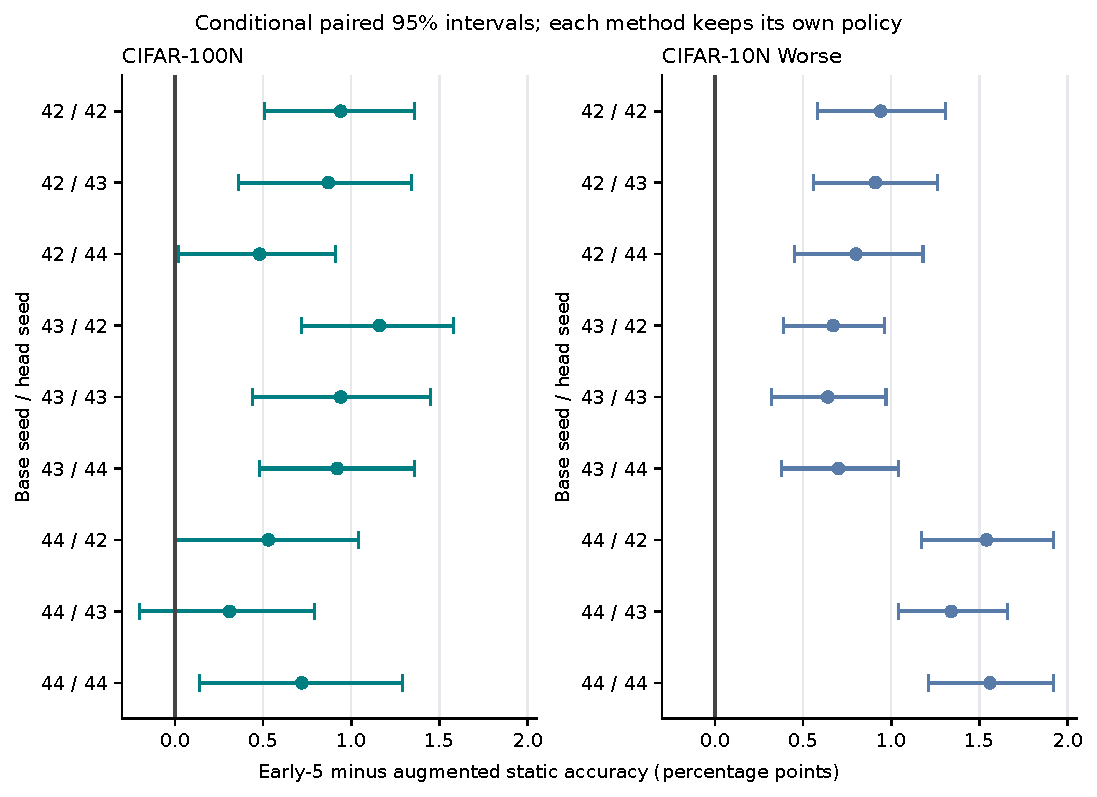
\includegraphics[width=\linewidth]{figures/augmentation_control.pdf}
\caption{Early-5 minus augmented-static accuracy. Bars are nominal 95\% paired test-example intervals conditional on each fitted base/head and selected policy, without multiplicity correction. They do not estimate base-training uncertainty. The policies can select different view counts.}
\label{fig:augmentation_control}
\end{figure}

\clearpage
\section{Matched Inference Microbenchmark}
\label{app:runtime}
A single Tesla T4 session runs sequentially on CIFAR-100N base44 and CIFAR-10N base43 using PyTorch 2.11.0+cu128, FP32 and four CPU threads. Head seed42 is fixed. Each timing configuration uses five warmups and 30 synchronized repetitions. Batch sizes 1/4 and view counts 1/5/10 are predefined; images are the first four fixed noisy-validation IDs, with shared deterministic view prefixes. Neither accuracy nor labels select timing cases. Temperatures come from each saved view budget's validation policy, rather than the globally selected view count. This reference inference path fuses the selected base features, PCA and the scalar head; cache generation and model/disk loading are outside the timing scope.

Table~\ref{tab:runtime} reports batch-size-one medians. The model scope starts from device tensors; the preprocessing scope includes CPU view generation, normalization and host-to-device transfer. Full CSVs retain batch medians/p95, batch-four amortized cost and GPU allocation measurements. Batch-four p95 is not per-image p95. Peak MB means PyTorch-allocated CUDA memory in decimal MB, not total device memory. Uniform/single-view policies skip the head.

\begin{table}[!ht]
\centering\small
\caption{Single-image inference medians (ms), head42 on one T4. Peak MB is allocated memory for the preprocessing-inclusive scope. Comparisons use the same view budget; these are not independent timing replications.}
\label{tab:runtime}
\begin{tabular}{llrrrr}
\toprule
Run & Method & Views & Model ms & With prep. ms & Peak MB \\
\midrule
C100/44 & Base & 1 & 7.68 & 7.59 & 133.9 \\
C100/44 & Uniform & 5 & 15.86 & 20.25 & 161.4 \\
C100/44 & Early-5 & 5 & 15.89 & 20.36 & 166.3 \\
C100/44 & Uniform & 10 & 30.42 & 40.05 & 215.1 \\
C100/44 & Early-5 & 10 & 30.46 & 40.40 & 219.8 \\
C10/43 & Base & 1 & 6.51 & 7.52 & 133.2 \\
C10/43 & Uniform & 5 & 16.47 & 20.82 & 160.7 \\
C10/43 & Early-5 & 5 & 16.66 & 20.46 & 165.5 \\
C10/43 & Uniform & 10 & 31.80 & 40.93 & 214.3 \\
C10/43 & Early-5 & 10 & 31.94 & 41.01 & 219.1 \\
\bottomrule
\end{tabular}

\end{table}

At five/ten views the observed extra allocated peak memory is about 4.8 MB for the PCA/head. Multi-view prediction is substantially costlier than a one-view base pass. Close matched-view medians are preliminary: one session, a fixed measurement order, a tiny fixed image set, and no independent timing intervals preclude a precise overhead guarantee. Separate one-view cases using equivalent computations also exhibit timing variation. No two-base ensemble is timed. These results do not establish lower latency than an ensemble or the cost of separately returning a standalone error-ranking score for every image.
